% document formatting
\documentclass[10pt]{article}
\usepackage[utf8]{inputenc}
\usepackage[left=1in,right=1in,top=1in,bottom=1in]{geometry}
\usepackage[T1]{fontenc}
\usepackage{xcolor}

% math symbols, etc.
\usepackage{amsmath, amsfonts, amssymb, amsthm}

% lists
\usepackage{enumerate}

% images
\usepackage{graphicx} % for images
\usepackage{tikz}
\usetikzlibrary{intersections, calc}

% code blocks
% \usepackage{minted, listings} 

% verbatim greek
\usepackage{alphabeta}

\newcommand{\opt}{\texttt{OPT}}

\graphicspath{{./assets/images/Week 12}}

\title{02-613 Week 12 \\ \large{Algorithms and Advanced Data Structures}}
 
\author{Aidan Jan}

\date{\today}

\begin{document}
\maketitle

\section*{Proving Min Cut Max Flow}
We covered max flow and the Ford-Fulkerson Algorithm previously.  Now, we can define a cut through a graph.  A cut in undirected $G = (V, E)$ divides $G$ into partitions $A$ and $B = V \setminus A$.  The \textbf{weight} of a cut is
\[\sum_{a \in A, b \in B, (a, b) \in E} w(a, b)\]
An $st$-cut is a cut with $s \in A, t \in B$.  The \textbf{capacity} of a cut is
\[\sum_{a \in A, b \in B, (a, b) \in E} c(a, b)\]
The concept of having a \textit{min} cut is important because it is the same problem as max flow.  We can show this with a quick proof.\\\\
\textbf{Theorem 1:} let $f$ be an $st$ flow, and let $(A, B)$ be an $st$ cut.  Then, the value of the flow
\[v(f) = f^{out}(A) - f^{in}(A)\]
\textbf{Proof 1:} any flow that leaves $A$ must either return or flow to $t$.\\\\
\textbf{Theorem 2:} let $f$ be an $st$ flow, and let $(A, B)$ be an $st$ cut.  Then,
\[v(f) \leq \text{capacity}(A, B)\]
\textbf{Proof 2:} 
\begin{align*}
    v(f) &= f^{out}(A) - f^{in}(A) \\
    &\leq f^{out}(A) \\
    &= \sum_{e \in \text{cut}(A)} f(e) \\
    &\leq \sum_{e \in \text{cut}(A)} c(e) - \text{capacity}(A, B)
\end{align*}
Now, consider $f^*$ returned by Ford-Fulkerson, and let $G_{f^*}$ be the residual graph for $f^*$.  Then,
\[V(f^*) = \text{capacity}(A^*, B^*) = V(\hat{f})\]
From this, we get that the value of the max flow in any flow graph is equal to the capacity of the minimum cut.\\\\
The \textbf{Edmunds-Karp} algorithm is the one which solves min cut.  This one can be run in O($nm^2$).

\section*{Reductions to Max Flow}
A \underline{reduction} rewrites a problem in terms of another.  To ``reduce'' $A$ into $B$ means getting a solution for $B$ leads to a solution to $A$.  We will be using this technique to solve many problems.

\subsection*{Maximum Bipartite Matching}
Maximum bipartite matching is, given a bipartite graph $G = L \cup R, E$, find $S \subseteq E \subseteq L \times R$ that is as large as possible.  What this essentially means, is imagine each node on the left being a person, and each node on the right being a task.  The edges connecting them represent the person knows how to do the task.  We want to assign tasks such that as many tasks as possible may be completed.\\\\
To reduce this to max flow, we can add a source node to all the nodes in $L$, and a sink to all the nodes in $R$.  Let all the edges in the entire graph (including from source, and to sink), have a capacity of $1$.  This is because every node on the left needs to be paired to a node on the right.  Now we can call Ford-Fulkerson on this.\\\\
Now, we have to explain how it is correct.  Basically, Ford-Fulkersons stops running when there are no more valid paths from the source to the sink, which implies that as many tasks as possible must be taken up.  If there was a pairing that could have been added, then Ford-Fulkerson's would have found it, so having a pairing not found leads to a contradiction.\\\\
Finally, we can extract the matching from Ford Fulkerson by looking at which connections between the left and right are filled.\\\\
The runtime of this algorithm is the runtime of Ford-Fulkerson's, which would be O($m^2$).  In our graph, we have $n + 2$ vertices (matching, plus source and sink), $m + n$ edges (since we added $n$ edges connecting the source to all `left' vertices and sink to all `right' vertices), and a maximum cost of $m + n$.  Since the runtime of Ford Fulkerson is O($|E||C|$), our runtime would be O($(m + n)(m + n)$) = O($m^2$).

\subsection*{Supply and Demand}
Let $G$ be a graph where we have supply nodes, and demand nodes.  Edges have a capacity which represents the maximum product that could travel through the edge.  We want to decide whether or not all the demand can be filled.
\begin{itemize}
	\item First, compare the demand and the supply.  If the total supply is less than the total demand, we can't.
	\item Next, we can add a source node connecting to all the supply nodes, where the edges have capacity of the supply node's supply.  Similarly, we can add a sink node connecting to all the demand nodes which the edges added are the demand.
	\item Now, we can run Ford Fulkerson.
	\item The maximum demand we can satisfy would be the result of Ford Fulkerson.
\end{itemize}

\section*{Linear Programming}
A \textbf{linear program} is a program that takes in constaints (linear equations), and finds values of variables that minimize an objective function.  For example, one such program may be able to take in the constraints of two variables, $\{x_1, x_2\}$:
\begin{itemize}
	\item $2x_1 + x_2 \leq 4$
	\item $x_2 \geq 1$
	\item $x_1 - x_2 >= -2$
\end{itemize}
Our objective function may be to minimize $-x_1 - x_2$.
\begin{center}
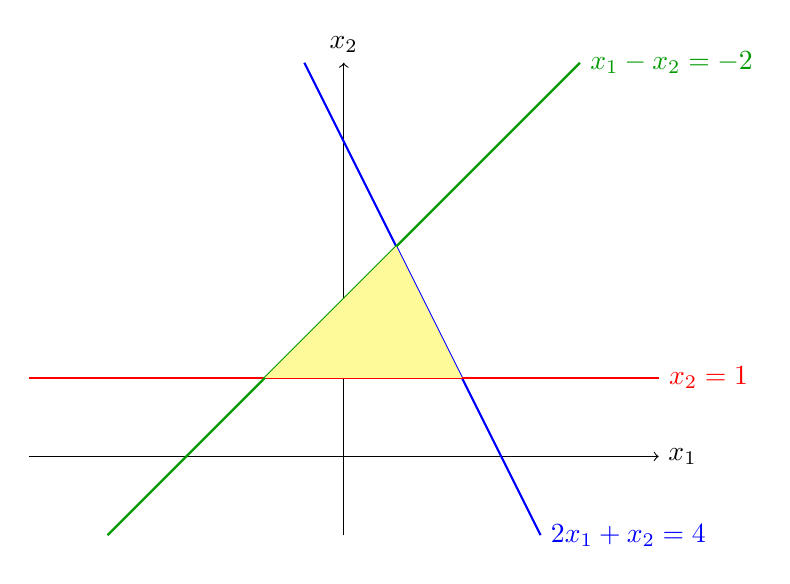
\begin{tikzpicture}[scale=1.0]

    % -------------------------
    % Axes
    % -------------------------
    \draw[->] (-4,0) -- (4,0) node[right] {$x_1$};
    \draw[->] (0,-1) -- (0,5) node[above] {$x_2$};

    % -------------------------
    % Constraint lines
    % -------------------------

    % 1) 2x1 + x2 = 4
    \draw[name path=C1, thick, blue]
        (-0.5, 5) -- (2.5, -1) node[right] {$2x_1 + x_2 = 4$};

    % 2) x2 = 1
    \draw[name path=C2, thick, red]
        (-4,1) -- (4,1) node[right] {$x_2 = 1$};

    % 3) x1 - x2 = -2   <=>  x1 = x2 - 2
    \draw[name path=C3, thick, green!60!black]
        (-3,-1) -- (3,5) node[right] {$x_1 - x_2 = -2$};

    % -------------------------
    % Shaded feasible region
    % -------------------------
    % We clip to a bounding box just for drawing visibility
    \begin{scope}
        \clip (-4,1) rectangle (4,5);   % ensures x2 ≥ 1
        \clip (-3, -1) -- (3, 5) -- (4,5) -- (4,-1) -- cycle;   % x1 ≤ x2 - 2
        \clip (-0.5, 5) -- (2.5,-1) -- (-4,-1) -- (-4,5) -- cycle;   % 2x1 + x2 ≤ 4

        \fill[yellow!40] (-4,1) rectangle (4,5);
    \end{scope}

\end{tikzpicture}
\end{center}
From here, the constraints makes our search space within the triangle, so we just find the point in the triangle that minimizes $-x_1 - x_2$.

\subsection*{Examples of Linear Solvers}
\begin{itemize}
	\item CPLEX
	\item Gurdoi
	\item Simplex
	\item Ellipsoid
	\item Interior Points
\end{itemize}

\subsection*{Why is this important?}
It turns that most of the problems covered before in this class can be written as linear programs.  For example, given a flow graph $G = (V, E)$ with capacities $c_e$, find a flow $f_e$ from $s \in V$ to $t \in V$ of max value, and each edge costs $p_e$ per unit.  In this case, we can have our objective to be to maximize 
\[\sum_{e \in E} f_e \cdot p_e\]
with constraints
\begin{itemize}
	\item $0 \leq f_e \leq c_e$
	\item $\sum_{(u, v) \in E} f(u, v) = \sum_{(v, w) \in E} f(v, w)$, $\forall v \in V, v \neq s, t$
\end{itemize}
We can then turn this into input for a linear program, and we get the solution to the problem without using Ford Fulkerson's.

\subsection*{Example: Shortest Path}
Given a directed graph $G = (V, E)$ with positive edge weights $w_k$, find the shortest path from $s \rightarrow t$.  Let
\[x_{uv} = \begin{cases} 1 & \text{if $(u, v)$ is in shortest path} \\ 0 & \text{otherwise} \end{cases}\]
The goal is to minimize $\sum x_{uv} \cdot w_{uv}$, while subject to
\begin{itemize}
    \item $\sum_{w:(u, t)} x_{ut} = 1$
    \item $\sum_{w:(s, v)} x_{sv} = 1$
    \item $\sum x_{uv} - \sum x_{vw} = 0 \quad \forall v \in V$
    \item $x_{uv} \in \{0, 1\}$
\end{itemize}
This can now be input into an LP.  There \textit{is} an important caveat though, which is here we are using integers.  It turns out that an LP can run in polynomial time, but an Integer LP (ILP) is NP-Complete.






\end{document}